% We switch to portrait mode. This works as advertised.
\documentclass[a0,portrait]{a0poster}
% You might find the 'draft' option to a0 poster useful if you have
% lots of graphics, because they can take some time to process and
% display. (\documentclass[a0,draft]{a0poster})

%\usepackage[utf8]{inputenc}

% Switch off page numbers on a poster, obviously, and section numbers too.
\pagestyle{empty}
\setcounter{secnumdepth}{0}

%fonts
\usepackage[T1]{fontenc}
\usepackage{kpfonts}
\usepackage{fontspec}
%\usepackage[oldstylenums, largesmallcaps]{kpfonts}
%\setmainfont[Numbers=OldStyle]{Tex Gyre Pagella}
\setmainfont{Tex Gyre Pagella}
\setsansfont[BoldFont=Lovelo-LineBold]{Lovelo-LineBold}
%\renewcommand*\sfdefault{ugq}

\usepackage{hyperref}
\hypersetup{%
	pdftitle={Wrinkling and nested buckling in a confined protein gel},%the title
	pdfauthor={Mathieu Leocmach},%your name
	hidelinks=true,
}

%proper math and math symbols
%\usepackage{amsmath}
\usepackage{amssymb}

\usepackage{siunitx}

\usepackage{multirow}

% Allow the usage of graphics (.jpg, .png, etc.) in the document
\usepackage{graphicx}
\usepackage{tikz}
\usetikzlibrary{arrows,shapes,backgrounds, positioning, intersections, decorations.markings, decorations.shapes, mindmap, shapes.geometric, matrix, patterns}

\usepackage{pgfplots}
%\usepgfplotslibrary{units}
\usepgfplotslibrary{groupplots}
\pgfplotsset{every axis/.append style={xlabel near ticks,ylabel near ticks,mark size={0.2em}}}
\pgfplotsset{every axis plot post/.append style={very thick}}

\usepgfplotslibrary{external}
%\tikzexternalize
%\tikzsetexternalprefix{fig_Rome/}
\tikzset{external/system call={lualatex \tikzexternalcheckshellescape -halt-on-error -interaction=batchmode -jobname "\image" "\texsource"}}

\usepackage{ragged2e}
\RaggedRight

\definecolor{Main}{rgb}{1, 0.57, 0}
\definecolor{Accent1}{rgb}{1,0.28,0}
\definecolor{Accent2}{rgb}{1,0.74,0}

% see documentation for a0poster class for the size options here
\let\Textsize\normalsize
\def\Norulehead#1{\noindent\hbox to \hsize{\hfil\LARGE\textcolor{Main}{\textsf{#1}}}\bigskip}
\def\Head#1{\Norulehead{\dotfill #1}}
\def\LHead#1{\noindent{\LARGE #1}\smallskip}
\def\Subhead#1{\noindent{\large\color{Accent1}\textsc{#1}}}
\def\Title#1{\noindent{\VeryHuge\color{Accent2}\raggedright\textsf{#1}}}

% The textpos package is necessary to position textblocks at arbitary 
% places on the page.
\usepackage[absolute,overlay,%showboxes
]{textpos}
% Set up the grid
%
% Note that [40mm,40mm] is the margin round the edge of the page --
% it is _not_ the grid size. That is always defined as 
% PAGE_WIDTH/HGRID and PAGE_HEIGHT/VGRID. In this case we use
% 15 x 25. This gives us a wide central column for text (7 grid
% spacings) and two narrow columns (3 each) at each side for 
% pictures, separated by 1 grid spacing.
%
% Note however that texblocks can be positioned fractionally as well,
% so really any convenient grid size can be used.
%
\TPGrid[40mm,40mm]{15}{25}  % 3 - 1 - 7 - 1 - 3 Columns

% Mess with these as you like
\parindent=0pt
%\parindent=1cm
\parskip=0.5\baselineskip

\usepackage{paralist}

%bibliography
\usepackage{natbib}
\usepackage{bibentry}
\def\newblock{\hskip .11em plus .33em minus .07em}



\newlength{\mylength}

%\includeonly{}

\begin{document}
%\tikzset{every mark/.append style={scale=0.8}}
%\pgfplotsset{every axis/.append style={small}}

\bibliographystyle{notitle}
%\nobibliography{sift}

% Understanding textblocks is the key to being able to do a poster in
% LaTeX. In
%
%    \begin{textblock}{wid}(x,y)
%    ...
%    \end{textblock}
%
% the first argument gives the block width in units of the grid
% cells specified above in \TPGrid; the second gives the (x,y)
% position on the grid, with the y axis pointing down.

% You will have to do a lot of previewing to get everything in the 
% right place.

% This gives good title positioning for a portrait poster.
% Watch out for hyphenation in titles - LaTeX will do it
% but it looks awful.
\begin{textblock}{15}(0,0)
\centering
\Title{
Wrinkling of a confined porous layer
}

\smallskip
\LHead{Mathieu Leocmach, Mathieu Nespoulous, Thomas Gibaud, Sébastien Manneville
}\hfill\texttt{\color{Accent1}mathieu.leocmach@ens-lyon.fr}\\

\LHead{\textsc{Laboratoire de Physique, Ecole Normale Supérieure de Lyon}\hfill\raisebox{-1.5\baselineskip}{
	\includegraphics[height=2\baselineskip,clip=true, trim=6mm 14mm 6mm 0]{NEW-Logo-ERC-OUTLINE}\quad
	\includegraphics[height=2\baselineskip]{logo_ums_grand}\quad
	\includegraphics[height=2\baselineskip]{CNRSfilaire-Q}\quad
	\includegraphics[height=2\baselineskip]{logo_ens-lyon}
}}

\end{textblock}

\begin{textblock}{3}(0,2.5)
	\Head{Acid-induced gels}
	
	Milk protein solution (4\%w sodium caseinate) acidified by the slow hydrolysis of glucono-$\delta$-lactone (4\%w \textsc{gdl})
	
	\begin{tikzpicture}
	\begin{groupplot}[%
		group style={
			group name=g, group size=1 by 2,
			xticklabels at=edge bottom,
			vertical sep=0,
			},
		xmin=0,xmax=8,
		scale only axis,
		width=\textwidth-4em,
		height=0.3\textwidth,
		extra tick style={grid=major},%
		ylabel absolute, every axis y label/.append style={anchor=base, yshift=1.25em}
		]
	\nextgroupplot[
		ymin=0, ymax=7, ylabel={\textcolor{Accent1}{pH}},
		extra y ticks={4.6}, extra y tick labels={},%
		]
	\addplot+[no marks,Accent1] table[x expr={\thisrowno{0}/3600.+0.05}]{Y189_28800s.pH};
	\node[base left=0] at (axis cs:8,4.6) {isoelectric};

	\nextgroupplot[
		xlabel={time (h)},
		ymin=0, ylabel=\textcolor{Accent2}{$G^\prime$ (\si{\pascal})}
		]
	\addplot+[no marks,Accent2] table[x expr={\thisrowno{0}/3600.+0.05}]{Y235_28800s.prise};
	\end{groupplot}
	\end{tikzpicture}
	
\Subhead{Confocal microscopy}\\ 10\% labelled casein
\end{textblock}

\begin{textblock}{7}(4,2.5)
	\Head{Sealed cell, spontaneous pattern}
	
	%\Subhead{Side view}\\
	\tikzsetnextfilename{cell_brushes}
	\tikzset{external/force remake}
	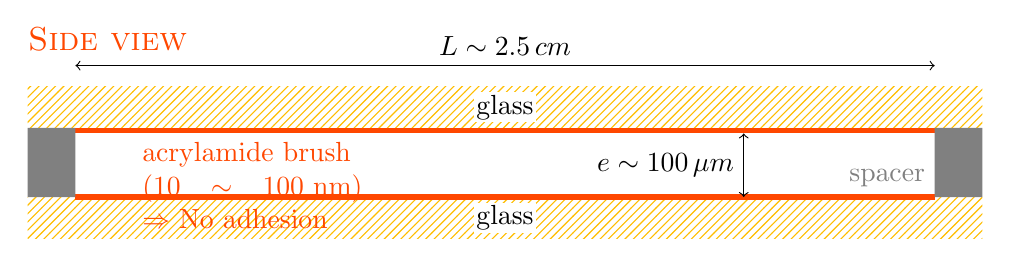
\begin{tikzpicture}
		\fill[pattern=north east lines,pattern color=Accent2] (0,0) rectangle (\textwidth,1.5em) node[midway,fill=white,inner sep=1pt] {glass};
		\fill[pattern=north east lines,pattern color=Accent2] (0,-2.5em) rectangle (\textwidth,-4em) node[midway,fill=white,inner sep=1pt] {glass};
		\draw[line width=2pt,Accent1] (0.05\textwidth,-2.5em) -- (0.95\textwidth,-2.5em) (0.05\textwidth,-1pt) -- (0.95\textwidth,-1pt) node[below,pos=0.30, text width=0.4\textwidth] {acrylamide brush ($10\sim 100$ nm)\linebreak $\Rightarrow$ No adhesion};
		\fill[gray] (0,0) rectangle (0.05\textwidth,-2.5em) (\textwidth,0) rectangle (0.95\textwidth,-2.5em) node[pos=1, above left] {spacer};
		\draw[<->] (0.75\textwidth,-2pt) -- (0.75\textwidth,-2.5em) node[midway,left] {$e\sim 100\,\mu m$};
		\draw[<->] (0.05\textwidth,2.25em) -- (0.95\textwidth,2.25em) node[midway,above] (L){$L\sim 2.5\,cm$};
		\node[anchor=north west, inner sep=0] at ($(L.north) - (0.5\textwidth,0)$) {\Subhead{Side view}};
	\end{tikzpicture}
	
	\Subhead{Top view}\\
	\begin{tikzpicture}[inner sep=0, very thick]
	\setlength{\mylength}{\columnwidth}
	\node[anchor=north west] (a) {\includegraphics[width=0.28\mylength]{cas3p2_fluo0p8_GDL4_50um_coating_2_zoom2_crop}};
		\node[anchor=north] at (0.44\mylength,0) (b) {\includegraphics[width=0.28\mylength]{cas3p2_fluo0p8_GDL4_50um_coating_2_zoom6_crop}};
		\node[anchor=north east] at (\mylength,0) (c) {\includegraphics[width=0.4\mylength]{cas3p2_fluo0p8_GDL4_50um_coating_2_transmission}};
		%zooms
		\node[minimum width = 0.137\mylength, minimum height=0.137\mylength, anchor=north west, draw=Accent2] at ($(a.north west) +(0.111\mylength,-0.072\mylength)$) (bz){};
		\draw[Accent2] (bz.north east) -- (b.north west) (bz.south east) -- (b.south west);
		\node[minimum width = 0.128\mylength, minimum height=0.081\mylength, anchor=north west, draw=Main] at ($(b.north west) +(0.097\mylength,-0.143\mylength)$) (cz){};
		\draw[Main] (cz.north east) -- (c.north west) (cz.south east) -- (c.south west);
		\node[minimum width = 0.156\mylength, minimum height=0.156\mylength, anchor=north west, draw=Accent1] at ($(c.north west) + (0.125\mylength,0)$) (dz) {};
		%scale bars
		\draw[ultra thick] (a.south east) ++(0,-0.25em) -- ++(-0.178\mylength,0) node[pos=0.5, below=0.25em, font=\small] (M) {\SI{1}{\centi\metre}};
		\draw[ultra thick] (b.south east) ++(0,-0.25em) -- ++(-0.176\mylength,0) node[pos=0.5, below=0.25em, font=\small] {\SI{5}{\milli\metre}};
		\draw[ultra thick] (c.south east) ++(0,-0.25em) -- ++(-0.132\mylength,0) node[pos=0.5, below=0.25em, font=\small] {\SI{1}{\milli\metre}};
		
		%final volumic view
		%\node[anchor=north east] at (\columnwidth,0) (c) {\includegraphics[width=0.4\mylength]{recol_volume_plis}};
	\end{tikzpicture}

\end{textblock}

\begin{textblock}{15}(0,8)
	\Head{Dynamics: wrinkling patterns and nested buckling}
	%\Head{No initial contact with a substrate: Poiseuille vs Darcy on a flying carpet}
	\begin{tikzpicture}
	\matrix[matrix of nodes, inner sep=0, column sep=0.015\textwidth, row sep=0.5em] (m){
	33 min & 38 min & 43 min & 48 min & 1h & 1h15 & 2h30\\
	\includegraphics[width=0.13\textwidth]{prise_0100_color.jpg}&
	\includegraphics[width=0.13\textwidth]{prise_0130_color.jpg}&
	\includegraphics[width=0.13\textwidth]{prise_0160_color.jpg}&
	\includegraphics[width=0.13\textwidth]{prise_0190_color.jpg}&
	\includegraphics[width=0.13\textwidth]{prise_0250_color.jpg}&
	\includegraphics[width=0.13\textwidth]{prise_0360_color.jpg}&
	\includegraphics[width=0.13\textwidth]{prise_0799_color.jpg}\\
	\includegraphics[width=0.13\textwidth]{cas3p2_fluo0p8_GDL4_2_t047_crop_resized.jpg}&
	\includegraphics[width=0.13\textwidth]{cas3p2_fluo0p8_GDL4_2_t056_crop_resized.jpg}&
	\includegraphics[width=0.13\textwidth]{cas3p2_fluo0p8_GDL4_2_t065_crop_resized.jpg}&
	\includegraphics[width=0.13\textwidth]{cas3p2_fluo0p8_GDL4_2_t074_crop_resized.jpg}&
	\includegraphics[width=0.13\textwidth]{cas3p2_fluo0p8_GDL4_2_t092_crop_resized.jpg}&
	\includegraphics[width=0.13\textwidth]{cas3p2_fluo0p8_GDL4_2_t125_crop_resized.jpg}&
	\includegraphics[width=0.13\textwidth]{cas3p2_fluo0p8_GDL4_2_t260_crop_resized.jpg}\\
	};
	\draw[ultra thick] ++(m-2-1.south west) -- ++(0.023\textwidth,0);
	\draw[ultra thick] ++(m-3-1.south west) -- ++(0.1\textwidth,0);
	\end{tikzpicture}
\end{textblock}




\begin{textblock}{7}(0,11)
	\Head{Synæresis and swelling cause buckling}
\end{textblock}

\begin{textblock}{3}(0,11.5)
\Subhead{Initial contact with a substrate}\\
	\begin{tikzpicture}
	\matrix[matrix of nodes, matrix anchor=north east, inner sep=0, row sep=0.01\textwidth]  (m){
	\includegraphics[width=\columnwidth, height=0.061\columnwidth]{coupe_cloque_t000.png}\\
	\includegraphics[width=\columnwidth, height=0.061\columnwidth]{coupe_cloque_t011.png}\\
	\includegraphics[width=\columnwidth, height=0.061\columnwidth]{coupe_cloque_t110.png}\\
	\includegraphics[width=\columnwidth, height=0.061\columnwidth]{coupe_cloque_t116.png}\\
	\includegraphics[width=\columnwidth, height=0.061\columnwidth]{coupe_cloque_t117.png}\\
	\includegraphics[width=\columnwidth, height=0.061\columnwidth]{coupe_cloque_t123.png}\\
	\includegraphics[width=\columnwidth, height=0.061\columnwidth]{coupe_cloque_t200.png}\\
	\includegraphics[width=\columnwidth, height=0.061\columnwidth]{coupe_cloque_t221.png}\\
	};
	\begin{scope}[above left, white, fill=gray, inner ysep=0]
		\node at (m-1-1.south east) {\SI{15}{\minute}};
		\node at (m-2-1.south east) {\SI{22}{\minute}};
		\node at (m-3-1.south east) {\SI{1}{\hour}~26};
		\node at (m-4-1.south east) {\SI{1}{\hour}~30};
		\node at (m-5-1.south east) {\SI{1}{\hour}~31};
		\node at (m-6-1.south east) {\SI{1}{\hour}~35};
		\node at (m-7-1.south east) {\SI{2}{\hour}~25};
		\node at (m-8-1.south east) {\SI{2}{\hour}~40};
	\end{scope}
	\draw[<->, ultra thick] ($(m-8-1.south west)+(0,-0.25em)$) -- +(0.786\textwidth,0) node[midway, below] {\SI{1}{\milli\metre}};
	\end{tikzpicture}
	
Cascade buckling \textit{Roman \& Pocheau 1999}

\Subhead{No initial contact}\\
\begin{tikzpicture}
	\matrix[matrix of nodes, matrix anchor=north east, inner sep=0, row sep=0.01\textwidth]  (m){
	\includegraphics[width=\columnwidth, height=0.052\columnwidth]{coupe_plis_t000.png}\\
	\includegraphics[width=\columnwidth, height=0.052\columnwidth]{coupe_plis_t016.png}\\
	\includegraphics[width=\columnwidth, height=0.052\columnwidth]{coupe_plis_t032.png}\\
	\includegraphics[width=\columnwidth, height=0.052\columnwidth]{coupe_plis_t038.png}\\
	\includegraphics[width=\columnwidth, height=0.052\columnwidth]{coupe_plis_t040.png}\\
	\includegraphics[width=\columnwidth, height=0.052\columnwidth]{coupe_plis_t043.png}\\
	\includegraphics[width=\columnwidth, height=0.052\columnwidth]{coupe_plis_t055.png}\\
	\includegraphics[width=\columnwidth, height=0.052\columnwidth]{coupe_plis_t070.png}\\
	\includegraphics[width=\columnwidth, height=0.052\columnwidth]{coupe_plis_t123.png}\\
	\includegraphics[width=\columnwidth, height=0.052\columnwidth]{coupe_plis_t332.png}\\
	};
	\begin{scope}[above left, white, fill=gray, inner ysep=0]
		\node at (m-1-1.south east) {\SI{15}{\minute}};
		\node at (m-2-1.south east) {\SI{23}{\minute}};
		\node at (m-3-1.south east) {\SI{32}{\minute}};
		\node at (m-4-1.south east) {\SI{35}{\minute}};
		\node at (m-5-1.south east) {\SI{36}{\minute}};
		\node at (m-6-1.south east) {\SI{38}{\minute}};
		\node at (m-7-1.south east) {\SI{44}{\minute}};
		\node at (m-8-1.south east) {\SI{53}{\minute}};
		\node at (m-9-1.south east) {\SI{1}{\hour}~21};
		\node at (m-10-1.south east) {\SI{3}{\hour}~15};
	\end{scope}
	\draw[<->, ultra thick] ($(m-10-1.south west)+(0,-0.25em)$) -- +(0.786\textwidth,0) node[midway, below] {\SI{1}{\milli\metre}};
	\end{tikzpicture}
	
	Globally unstable wavelength
\end{textblock}

\begin{textblock}{3}(4,11.5)
	\begin{tikzpicture}
	\begin{groupplot}[%
		group style={
			group name=g, group size=1 by 2,
			xticklabels at=edge bottom,
			vertical sep=0,
			},
		xmin=0, xmax=170, xtick={0,30,...,150},
		extra tick style={grid=major},%
		extra x ticks = {21,68}, extra x tick labels={},%
		scale only axis,
		width=\textwidth-4em,
		height=0.3\textwidth,
		ylabel absolute, every axis y label/.append style={anchor=base, yshift=1.25em}
		]
	
	\nextgroupplot[
		ylabel={Volume (\%)}, ymin=20, ymax=100, 
		ytick={40,60,80,100}, every axis y label/.append style={xshift=0.5em},
		]
	\addplot+[no marks,Accent1] table[x expr={\thisrowno{0}+15}, y expr={\thisrowno{1}*100}]{relative_volume_excess_area_cloques.txt};
	%\addplot+[only marks,Accent2, mark=+] table[y expr={\thisrowno{1}*100}]{volume_rel_half_cas8_toi.txt};
	\node[anchor=south west] at (rel axis cs:0,0) {\rotatebox{90}{synæresis}};
	\node at (axis cs:68,80) {swelling};
	
	\nextgroupplot[
		ylabel={Excess area (\%)}, ymin=0, ymax=4, ytick={0,1,2,3},
		xlabel={time (min)}, 
		every axis y label/.append style={xshift=-1em},
		]
	\addplot+[no marks,Accent1] table[x expr={\thisrowno{0}+15}, y expr={\thisrowno{2}*100}]{relative_volume_excess_area_cloques.txt} node[pos=1, below left] {all};
	\addplot+[no marks,Accent2] table[x expr={\thisrowno{0}+15}, y expr={\thisrowno{3}*100}]{relative_volume_excess_area_cloques.txt} node[pos=1, left] {single blister};
	\draw[->] (axis cs: 21, 3) -- (axis cs: 68, 3) node[midway, below] {\SI{1}{\hour}};
	%\legend{all, single blister};
	\end{groupplot}
	\end{tikzpicture}
	
	\begin{tikzpicture}
	\begin{groupplot}[%
		group style={
			group name=g, group size=1 by 2,
			xticklabels at=edge bottom,
			vertical sep=0,
			},
		xmin=0, xmax=180, xtick={0,30,...,150},
		extra tick style={grid=major},%
		extra x tick labels={},%
		scale only axis,
		width=\textwidth-4em,
		height=0.3\textwidth,
		ylabel absolute, every axis y label/.append style={anchor=base, yshift=1.25em}
		]
	
	\nextgroupplot[ylabel={Volume (\%)}, ymin=20, ymax=100, ytick={40,60,80,100}, every axis y label/.append style={xshift=0.5em}]
	\addplot+[no marks,Accent1] table[x expr={\thisrowno{0}+15}, y expr={\thisrowno{1}*100}]{relative_volume_excess_area_plis.txt};
	%\addplot+[only marks,Accent2, mark=+] table[y expr={\thisrowno{1}*100}]{volume_rel_half_cas8_toi.txt};
	
	\nextgroupplot[ylabel={Excess area (\%)}, ymin=0, ymax=6, ytick={0,2,4}, 
	xlabel={time (min)}, every axis y label/.append style={xshift=-1em}]
	\addplot+[no marks,Accent1] table[x expr={\thisrowno{0}+15}, y expr={\thisrowno{2}*100}]{relative_volume_excess_area_plis.txt};
	%\addplot+[only marks,Accent2, mark=+] table{excess_area_pc_half_cas8_toi.txt};
	\end{groupplot}
	\end{tikzpicture}
\end{textblock}






\begin{textblock}{3}(12,12)
\textit{Kolinski et al 2009, Vella et al 2009}\\
Bending energy $B$ vs vertical stress $\sigma$:
\[ \lambda^* = \left(\frac{B}{\sigma}\right)^{1/3}\text{, eg. }\sigma =\rho g h \]
\end{textblock}

\begin{textblock}{7}(8,11)
	\Head{Wavelength: resisting stress needed}
	\Subhead{Initial contact with a substrate : Ruck in a rug analogy}

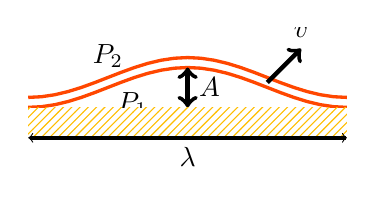
\begin{tikzpicture}[ultra thick]
\begin{axis}[
	name=a,
	width=3\TPHorizModule, height=0.75\TPHorizModule, scale only axis,
	domain=-180:180, no markers, ymin=0, ymax=4,xmin=-180,xmax=180,
	axis lines=none, xtick=\empty,
	]
	\addplot+[Accent1]{cos(x)+1};
	\addplot+[Accent1]{cos(x)+1.5};
	\draw[->, ultra thick] (axis cs:90,1.25) -- +(45:0.05\textwidth) node[pos=1, above] {$\vec{v}$};
	\node[above] at (axis cs:-90,1.5) {$P_2$};
	\node[below right] at (axis cs:-90,1.25) {$P_1$};
	\draw[<->, ultra thick] (axis cs:0,0) -- (axis cs:0,2) node[midway, right] {$A$};
\end{axis}
\fill[pattern=north east lines,pattern color=Accent2] (a.south west) rectangle ($(a.south east)+(0,-1em)$);
\draw[<->] ($(a.south west)+(0,-1.1em)$) -- ($(a.south east)+(0,-1.1em)$) node[midway, below] {$\lambda$};
\end{tikzpicture}

Actual shape depends on relative excess length $\epsilon$: $\lambda \sim \epsilon^{1/7} \lambda^*$ and $A \sim \epsilon^{4/7} \lambda^*$

\Subhead{Poroelasticity instead of gravity} \hfill Vertical cells show the same wavelength
\begin{itemize}
\item Solvent must flow through the gel(volumic flux $v\simeq \SI{0.2}{\micro\metre\per\second}$, pore size $\ell_p \approx \SI{4}{\micro\metre}$)
\item[$\Rightarrow$] $\sigma$ is a Darcy pressure
$\sigma = \Delta P \sim \eta h v/\ell_p^2   $
\hfill\fcolorbox{Main}{white}{$\Rightarrow$ Poroelastic length
$\displaystyle \lambda^* \sim \left(\frac{B \ell_p^2}{\eta v h}\right)^\frac{1}{3} \simeq \SI{2}{\milli\metre}$}
\item Different from usual poroelasticity (\textit{Biot 1964}) where pore pressure increases transiently the bending energy. Here Darcy flow resists large wavelength.
\end{itemize}

\Subhead{No initial contact with a substrate: Poiseuille vs Darcy on a flying carpet}

\smallskip
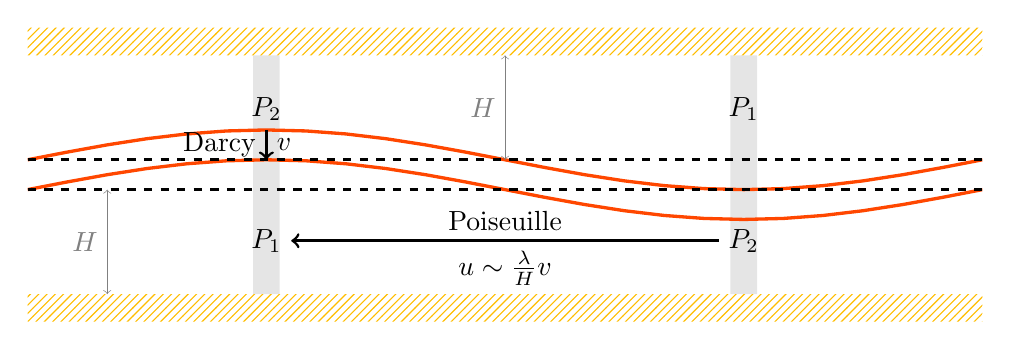
\begin{tikzpicture}
\begin{axis}[
	name=a,
	width=\textwidth, height=0.25\textwidth, scale only axis,
	domain=0:360, no markers, ymin=-4, ymax=4,xmin=0,xmax=360,
	axis lines=none, xtick=\empty,
	]
	\fill[gray!20] (axis cs:85,4) rectangle (axis cs:95,-4) (axis cs:265,4) rectangle (axis cs:275,-4);
	\addplot+[Accent1]{sin(x)+0.5};
	\addplot+[Accent1]{sin(x)-0.5};
	\addplot+[dashed, black]{0.5};
	\addplot+[dashed, black]{-0.5};
	\draw[<->, help lines] (axis cs:180,0.5) -- (axis cs:180,4) node[midway, left] {$H$}; 
	\draw[<->, help lines] (axis cs:30,-0.5) -- (axis cs:30,-4) node[midway, left] {$H$};
	\node[below] at (axis cs:90,-1.5) (pb1) {$P_1$};
	\node[above] at (axis cs:90,1.5) (ph2) {$P_2$};
	\node[above] at (axis cs:270,1.5) (ph1) {$P_1$};
	\node[below] at (axis cs:270,-1.5) (pb2) {$P_2$};
	\draw[line width=0.1em, ->] (ph2) -- (axis cs:90,0.5) node[midway, left] {Darcy} node[midway, right] {$v$};
	\draw[line width=0.1em, ->] (pb2) -- (pb1) node[midway, above] {Poiseuille} node[midway, below] {$u \sim \frac{\lambda}{H} v$};
\end{axis}
\fill[pattern=north east lines,pattern color=Accent2] (a.south west) rectangle +(\textwidth,-1em) (a.north west) rectangle +(\textwidth,1em);
\end{tikzpicture}

\begin{itemize}
\item The same $\Delta P$ can be relaxed by a Poiseuille flow
$\Delta P \sim 12\eta\frac{\lambda}{H^2} u \sim 12\eta\frac{\lambda^2}{H^3} v$
\item For the same wavelength
$\frac{v_\text{Darcy}}{v_\text{Poiseuille}} \sim \frac{\ell_p^2\lambda^2}{hH^3} \approx 30$ \hfill$\Rightarrow$ Flow through the pores dominates
\end{itemize}
\end{textblock}

\begin{textblock}{7}(0,18)
	\Head{Cell thickness}
\begin{tikzpicture}[mark size={0.3em}]
	\matrix[matrix of nodes, inner sep=0, column sep=0.01\columnwidth, row sep=0.01\columnwidth] (m) {
		\includegraphics[width=0.245\columnwidth]{pattern_50um.jpg}&
		\includegraphics[width=0.245\columnwidth]{pattern_100um.jpg}&
		\includegraphics[width=0.245\columnwidth]{pattern_250um.jpg}&
		\includegraphics[width=0.245\columnwidth]{pattern_450um.jpg}\\
	};
	\node[inner sep=0, below left=0.01\columnwidth and 0 of m.south east] (x800) {\includegraphics[width=0.49\columnwidth]{pattern_800um_x1.jpg}};
	\draw[ultra thick, Accent2, <->] (x800.south west) ++(0.196\columnwidth, 0.05\columnwidth) -- ++(0.145\columnwidth,0) node[midway,above]{$\lambda$};
	\draw[line width=0.2em,Main](x800.north east) -- ++(-0.217\columnwidth,0) node[midway,below] {\SI{5}{\milli\metre}};
	
	\begin{axis}[%
		name=g,
		anchor=left of north west,
		at={($(m.south west)+(0,-0.01\columnwidth)$)},
		scale only axis,
		width=3\TPHorizModule-4em,
		height=0.25\columnwidth-2em,
		xmin=0,xmax=1,xlabel={gap (\si{\milli\metre})},
		xtick={0,0.4,...,0.9},
		ymin=0,ylabel={$\lambda$ (\si{\milli\metre})},
		ylabel absolute, every axis y label/.append style={anchor=base, yshift=1.25em},
		cycle multi list={%
			Accent1,no marks\\%
			Accent1,only marks,every mark/.append style={fill=Accent1},mark=*\\%
			Accent1,only marks,every mark/.append style={fill=white},mark=*\\%
			Accent1,only marks,every mark/.append style={fill=Accent1},mark=triangle*\\%
			Accent1,only marks,every mark/.append style={fill=white},mark=triangle*\\%
			Accent1,only marks,every mark/.append style={fill=Accent1},mark=square*\\%
			Accent1,only marks,every mark/.append style={fill=white},mark=square*\\%
		},
		mark size={0.3em}
		]
		\addplot+[domain=0:3] {4.23*x};
		\addplot coordinates {(0.05,0.261)};\label{pgfplots:50}
		\addplot coordinates {(0.1,0.458)};\label{pgfplots:100}
		\addplot coordinates {(0.250,0.916)};\label{pgfplots:250}
		\addplot coordinates {(0.450,2.075)};\label{pgfplots:450}
		\addplot coordinates {(0.800,3.333)};\label{pgfplots:800}
		%\addplot+[only marks,Accent1, mark options={fill=Accent1}] coordinates {(0.05,0.261) (0.1,0.458) (0.250,0.916) (0.450,2.075) (0.800,3.333)};
	\end{axis}
	\node[below right=0 of m-1-1.north west] {\ref{pgfplots:50}};
	\node[below right=0 of m-1-2.north west] {\ref{pgfplots:100}};
	\node[below right=0 of m-1-3.north west] {\ref{pgfplots:250}};
	\node[below right=0 of m-1-4.north west] {\ref{pgfplots:450}};
	\node[below right=0 of x800.north west] {\ref{pgfplots:800}};
\end{tikzpicture}

\Subhead{Wavelength stop evolving after a blister touches the ceiling}
\end{textblock}


\begin{textblock}{3}(0,22.25)
	\begin{tikzpicture}
\begin{axis}[
	scale only axis,
	width=\textwidth-4em,
	height=0.4\textwidth,
	xmin=0, xmax=1000, xtick={0,250, 500, 750}, xlabel={position (\si{\micro\metre})},
	ymin=0, ymax=50, ylabel={altitude (\si{\micro\metre})},
	ylabel absolute, every axis y label/.append style={anchor=base, yshift=1.25em},
	cycle list={
		{Accent2}, 
		{black!15!Accent2},
		{black!30!Accent2},
		{black!45!Accent2},
		{black!60!Accent2},
		{black!75!Accent2},
		{black}
	},
	no marks,
	]
	\foreach \x in {2,3,..., 8}
		\addplot table[y index=\x]{alts_bottom_cloque.txt};
		
	\draw[ultra thick, Accent1] (axis cs:580,0) -- (axis cs:580,50);
\end{axis}
\end{tikzpicture}
\end{textblock}

\begin{textblock}{3}(4,22.25)
At contact: $A=H\equiv e-h\approx e/2$
	\[ \lambda \sim \epsilon^{-3/7} H \]
	\[ \epsilon \sim \left(\frac{\lambda}{e}\frac{e}{H}\right)^{-7/3} \simeq 0.6\% \]
	
\end{textblock}



\begin{textblock}{7}(8,21)
\Head{Surprising viscosity influence}
\begin{tikzpicture}
	\begin{loglogaxis}[%
		scale only axis,
		width=3\TPHorizModule-4em,
		height=2\TPHorizModule,
		xmin=0.6,xmax=11,xlabel={viscosity (\si{\milli\pascal\second})},
		xtick={0.7, 1, 2, 5, 10}, xticklabels={$0.7$, $1$, $2$, $5$, $10$},
		ytick={1,2,3,4}, yticklabels={$1$,$2$,$3$,$4$},
		ymin=1, ymax=5, ylabel={$\lambda$ (\si{\milli\metre})},
		ylabel absolute, every axis y label/.append style={anchor=base, yshift=1.25em},
		mark size={0.3em},
		legend style={legend pos=south east},
		]
		\addplot+[no marks, domain=0.7:10, black, forget plot] {1.7*x^0.4} node[midway, below] {$\eta^{0.4}$};
		\addplot+[only marks,Accent1, mark options={fill=Accent1}] table{eta_lambda_eau_pure.txt};
		\addplot+[only marks,Accent2, mark options={fill=Accent2}] table{eta_lambda_eau_glycerol.txt};
		\legend{water, water-glycerol};
	\end{loglogaxis}
\end{tikzpicture}
\end{textblock}

\begin{textblock}{3}(12,21.5)
\begin{itemize}
\item $\lambda$ increases with $\eta$
\item Can be explained only by a hidden dependence of $\eta$ on $B$, $\ell_p$, \ldots 
\item[\Rightarrow] Viscosity influences gel formation.
\end{itemize}
If $\ell_p \sim \eta^{-\alpha}$ and $B\sim \mathrm{k_B}T \left(\frac{h}{\ell}\right)^3$, then
\[ \lambda^* \sim \eta^\frac{\alpha-1}{3} \]
\[\alpha\simeq 2.2\]
\end{textblock}


\begin{textblock}{15}(0,24.75)
\small{\texttt{The research leading to these results has received funding from the European Research Council under the European Union's Seventh Framework Programme (FP7/2007-2013) / ERC grant agreement n°~258803.}}
\end{textblock}


\textblockcolour{lightgray!50!white}
\TPMargin*{ 0.125\TPHorizModule }
\begin{textblock}{2.875}(12,2.625)%real width of 3
	\Norulehead{Take home}
	\Subhead{Original patterns}
	\begin{itemize}
		\item nested (optical elements ?)
		\item generated by swelling
		\item kinetic wavelength selection
	\end{itemize}
	\Subhead{A new wrinkling mechanism}
	\begin{itemize}
		\item porous flow resist bending
		\item Darcy can beat Poiseuille
		\item may extend to other porous sheets 
		\begin{itemize}
			\item wet paper
			\item biological membranes
		\end{itemize}
	\end{itemize}
	\Subhead{Viscosity influences}
	\begin{itemize}
		\item porous dissipation, thus wrinkling
		\item gel formation, thus wrinkling
	\end{itemize}
	

\end{textblock}%Conclusion



\end{document}